\documentclass[14pt]{extbook}
\usepackage{multicol, enumerate, enumitem, hyperref, color, soul, setspace, parskip, fancyhdr} %General Packages
\usepackage{amssymb, amsthm, amsmath, latexsym, units, mathtools} %Math Packages
\everymath{\displaystyle} %All math in Display Style
% Packages with additional options
\usepackage[headsep=0.5cm,headheight=12pt, left=1 in,right= 1 in,top= 1 in,bottom= 1 in]{geometry}
\usepackage[usenames,dvipsnames]{xcolor}
\usepackage{dashrule}  % Package to use the command below to create lines between items
\newcommand{\litem}[1]{\item#1\hspace*{-1cm}\rule{\textwidth}{0.4pt}}
\pagestyle{fancy}
\lhead{Progress Quiz 7}
\chead{}
\rhead{Version C}
\lfoot{4173-5738}
\cfoot{}
\rfoot{Spring 2021}
\begin{document}

\begin{enumerate}
\litem{
To estimate the one-sided limit of the function below as $x$ approaches 4 from the left, which of the following sets of numbers should you use?\[ \frac{\frac{4}{x} - 1}{x - 4} \]\begin{enumerate}[label=\Alph*.]
\item \( \{ 3.9000, 3.9900, 3.9990, 3.9999 \} \)
\item \( \{ 4.0000, 4.1000, 4.0100, 4.0010 \} \)
\item \( \{ 4.1000, 4.0100, 4.0010, 4.0001 \} \)
\item \( \{ 4.0000, 3.9000, 3.9900, 3.9990 \} \)
\item \( \{ 3.9000, 3.9900, 4.0100, 4.1000 \} \)

\end{enumerate} }
\litem{
Evaluate the one-sided limit of the function $f(x)$ below, if possible.\[ \lim_{x \rightarrow 6^+} \frac{6}{(x-6)^6}+5 \]\begin{enumerate}[label=\Alph*.]
\item \( \infty \)
\item \( f(6) \)
\item \( -\infty \)
\item \( \text{The limit does not exist} \)
\item \( \text{None of the above} \)

\end{enumerate} }
\litem{
Evaluate the one-sided limit of the function $f(x)$ below, if possible.\[ \lim_{x \rightarrow -5^-} \frac{6}{(x-5)^9}+4 \]\begin{enumerate}[label=\Alph*.]
\item \( f(-5) \)
\item \( -\infty \)
\item \( \infty \)
\item \( \text{The limit does not exist} \)
\item \( \text{None of the above} \)

\end{enumerate} }
\litem{
For the graph below, find the value(s) $a$ that makes the statement true: $ \displaystyle \lim_{x \rightarrow a} f(x) = -\infty$.
\begin{center}
    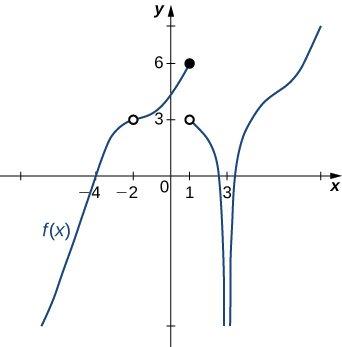
\includegraphics[width=0.5\textwidth]{../Figures/evaluateLimitGraphicallyCopyC.png}
\end{center}
\begin{enumerate}[label=\Alph*.]
\item \( -2 \)
\item \( -\infty \)
\item \( 3 \)
\item \( \text{Multiple } a \text{ make the statement true}. \)
\item \( \text{No } a \text{ make the statement true}. \)

\end{enumerate} }
\litem{
Evaluate the limit below, if possible.\[ \lim_{x \rightarrow 9} \frac{\sqrt{5x - 20} - 5}{9x - 81} \]\begin{enumerate}[label=\Alph*.]
\item \( 0.011 \)
\item \( 0.100 \)
\item \( \infty \)
\item \( 0.248 \)
\item \( \text{None of the above} \)

\end{enumerate} }
\litem{
Evaluate the limit below, if possible.\[ \lim_{x \rightarrow 6} \frac{\sqrt{8x - 23} - 5}{3x - 18} \]\begin{enumerate}[label=\Alph*.]
\item \( 0.943 \)
\item \( 0.267 \)
\item \( 0.100 \)
\item \( \infty \)
\item \( \text{None of the above} \)

\end{enumerate} }
\litem{
To estimate the one-sided limit of the function below as $x$ approaches 8 from the left, which of the following sets of numbers should you use?\[ \frac{\frac{8}{x} - 1}{x - 8} \]\begin{enumerate}[label=\Alph*.]
\item \( \{ 8.1000, 8.0100, 8.0010, 8.0001 \} \)
\item \( \{ 8.0000, 7.9000, 7.9900, 7.9990 \} \)
\item \( \{ 7.9000, 7.9900, 8.0100, 8.1000 \} \)
\item \( \{ 8.0000, 8.1000, 8.0100, 8.0010 \} \)
\item \( \{ 7.9000, 7.9900, 7.9990, 7.9999 \} \)

\end{enumerate} }
\litem{
For the graph below, find the value(s) $a$ that makes the statement true: $ \displaystyle \lim_{x \rightarrow a} f(x) = 0$.
\begin{center}
    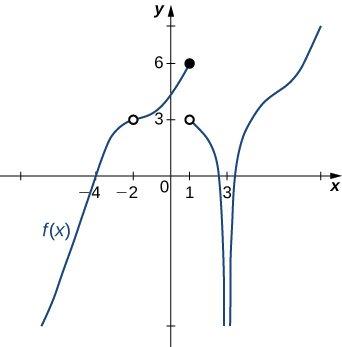
\includegraphics[width=0.5\textwidth]{../Figures/evaluateLimitGraphicallyC.png}
\end{center}
\begin{enumerate}[label=\Alph*.]
\item \( 3 \)
\item \( 0 \)
\item \( -4 \)
\item \( \text{Multiple } a \text{ make the statement true}. \)
\item \( \text{No } a \text{ make the statement true}. \)

\end{enumerate} }
\litem{
Based on the information below, which of the following statements is always true?
\begin{center}
    \textit{ $f(x)$ approaches $17.121$ as $x$ approaches $7$. }
\end{center}
\begin{enumerate}[label=\Alph*.]
\item \( f(17) = 7 \)
\item \( f(7) = 17 \)
\item \( f(7) \text{ is close to or exactly } 17 \)
\item \( f(17) \text{ is close to or exactly } 7 \)
\item \( \text{None of the above are always true.} \)

\end{enumerate} }
\litem{
Based on the information below, which of the following statements is always true?
\begin{center}
    \textit{ $f(x)$ approaches $3.475$ as $x$ approaches $9$. }
\end{center}
\begin{enumerate}[label=\Alph*.]
\item \( f(x) \text{ is close to or exactly } 3.475 \text{ when } x \text{ is close to } 9 \)
\item \( f(x) = 3.475 \text{ when } x \text{ is close to } 9 \)
\item \( f(x) \text{ is close to or exactly } 9 \text{ when } x \text{ is close to } 3.475 \)
\item \( f(x) = 9 \text{ when } x \text{ is close to } 3.475 \)
\item \( \text{None of the above are always true.} \)

\end{enumerate} }
\end{enumerate}

\end{document}